\chapter{Methodology}
\label{ch:methodology}

This chapter describes the complete methodological pipeline developed for the reconstruction of EAS at CONDOR using deep learning. It covers the experimental conditions under which the data were generated, the construction and preprocessing of the dataset, the architecture of the proposed model, the strategy used to identify its optimal configuration, and the training procedure that resulted from that search. Together, these components constitute the full technical contribution of this thesis.

\section{Experimental Setup}

The experimental conditions of this work are determined by the design and operational constraints of the CONDOR observatory, described in detail in Section~\ref{sec:condor_observatory}, and the simulation framework introduced in Section~\ref{sec:corsika}. Because the observatory has not yet begun scientific operations, all data are generated through CORSIKA simulations configured to match CONDOR's geometry and high-altitude observation level of 5,300 m above sea level.

Two primary particle types are simulated, protons and gamma rays, at three discrete energies: 300, 500, and 800 GeV. This discrete sampling was a deliberate design choice to maintain adequate statistical representation per energy bin while limiting the overall computational cost of the simulation campaign, and it challenges the model to generalize to continuous energy values between training points. Zenith angles are sampled from $0\degree$ to $40\degree$ in steps of $2\degree$, producing 21 discrete inclinations, while the azimuthal angle is fixed at $\phi = 0$ for all simulations. This is a deliberate simplification that reduces the simulation cost and isolates the zenith-angle dependence. 

It should be noted that the array geometry offers little symmetry to lean on: in the proposed CONDOR layout, both the individual modules and the central grid they form are rectangular rather than square in their two horizontal dimensions, so the array maps onto itself only under a $180\degree$ rotation and possesses two-fold rather than four-fold or continuous rotational symmetry. The fixed azimuth therefore introduces a directional bias that is examined explicitly in Chapter~\ref{ch:results}. Events producing fewer than 30 secondary particles at the observation level are discarded, removing low-multiplicity cases that carry insufficient information for reliable reconstruction.

\section{Dataset Construction and Preprocessing}

The raw output of the CORSIKA simulations is particle-level: for each event it records the secondary particles reaching the observation level, with their ground positions, arrival times, and energies, rather than any notion of detector modules. The first preprocessing step aggregates these particle hits onto the 120 detector modules of the array, so that each event is subsequently described by the set of modules that registered at least one hit during the shower passage, together with the physical quantities recorded at each active module. The simulations employ the EPOS model~\shortcite{pierog2009epos} for high-energy hadronic interactions and the GHEISHA model~\shortcite{fesefeldt1985gheisha} for low-energy hadronic and electromagnetic processes, following the same configuration used by~\shortciteA{arratia2025condor}. Transforming this raw output into a structured representation suitable for deep learning requires two steps: the construction of a dual-input encoding that captures complementary aspects of each shower event, and the normalization of all input features to a common scale.

\textbf{Sequential Features.} The first input branch encodes the spatiotemporal development of the shower front across the detector array. For each event, all active detector hits are collected and sorted in ascending order of their recorded time bin. Each hit is represented as a six-dimensional vector containing the detector identifier, the particle count registered at that module, the time bin index $t_{\text{bin}}$, the total deposited energy $\varepsilon$, and the horizontal coordinates $x_{\text{center}}$ and $y_{\text{center}}$ of the module's position within the array. The resulting input for a single event is a matrix of shape $n \times 6$, where $n$ is the number of active detector hits ordered chronologically. This ordering is physically meaningful: the earliest hits correspond to the leading edge of the shower front, which carries the strongest directional signal, while later hits trace the lateral spread and tail of the shower development. Because $n$ varies across events, sequences are zero-padded to a common maximum length, and a boolean mask is passed alongside each sequence to prevent padded positions from contributing to the attention computation in the Transformer component.

\textbf{Global Features.} The second input branch encodes the aggregate properties of the event as a fixed-length vector of five statistics, in the exact order implemented in the preprocessing pipeline: (1) the total particle count summed across all modules, (2) the total deposited energy summed across all modules, (3) the number of active detectors, (4) the temporal duration of the event, defined as the difference between the last and first recorded time bins, and (5) the deposited energy recorded by the central detectors of the array. These quantities capture the overall scale and spatial extent of the shower without encoding its internal temporal structure, providing a complementary signal that is particularly informative for energy estimation, where the total shower size is more directly relevant than the sequence of individual hits. The exact computation and normalization of each global feature are detailed in Appendix~\ref{sec:apx_global_features}, and Table~\ref{tab:dual-input} illustrates the dual-input data structure and the physical meaning of each feature branch.
\begin{table}[ht!]
\centering
\small
\caption[Dual-input feature structure.]{Dual-input feature structure of the
CNN-Transformer model.}
\label{tab:dual-input}
\setlength{\tabcolsep}{8pt}
\renewcommand{\arraystretch}{1.15}
\begin{tabular}{llll}
\toprule
\textbf{Input} & \textbf{Shape} & \textbf{Feature} & \textbf{Description} \\
\midrule
\multirow{5}{*}{Sequential} & \multirow{5}{*}{$(n \times 6)$}
    & $\text{ID}_i$               & Detector identifier \\
 && $\text{count}_i$              & Particle count \\
 && $t_i$                         & Binned arrival time \\
 && $\varepsilon_i$               & Deposited energy \\
 && $x_i,\ y_i$                  & Detector coordinates \\
\midrule
\multirow{5}{*}{Global} & \multirow{5}{*}{$(5)$}
    & \texttt{total\_particles}   & Total particle count \\
 && \texttt{total\_energy}        & Total deposited energy \\
 && \texttt{active\_detectors}    & Active detector count \\
 && \texttt{duration}             & Shower duration \\
 && \texttt{central\_energy}      & Central array energy \\
\bottomrule
\multicolumn{4}{l}{%
    \footnotesize $n$: number of hits per event, padded to \texttt{maxlen};
    sequences masked at padded positions.}
\end{tabular}
\end{table}

Figure~\ref{fig:individual_events} shows representative individual events for each combination of particle type and primary energy, illustrating the variability in shower morphology at the single-event level. Figure~\ref{fig:footprint_grid} shows the corresponding average footprints, computed over roughly 770 events per cell, which suppress stochastic fluctuations and reveal the systematic morphological differences exploited by the model.

\begin{figure}[!ht]
    \centering
    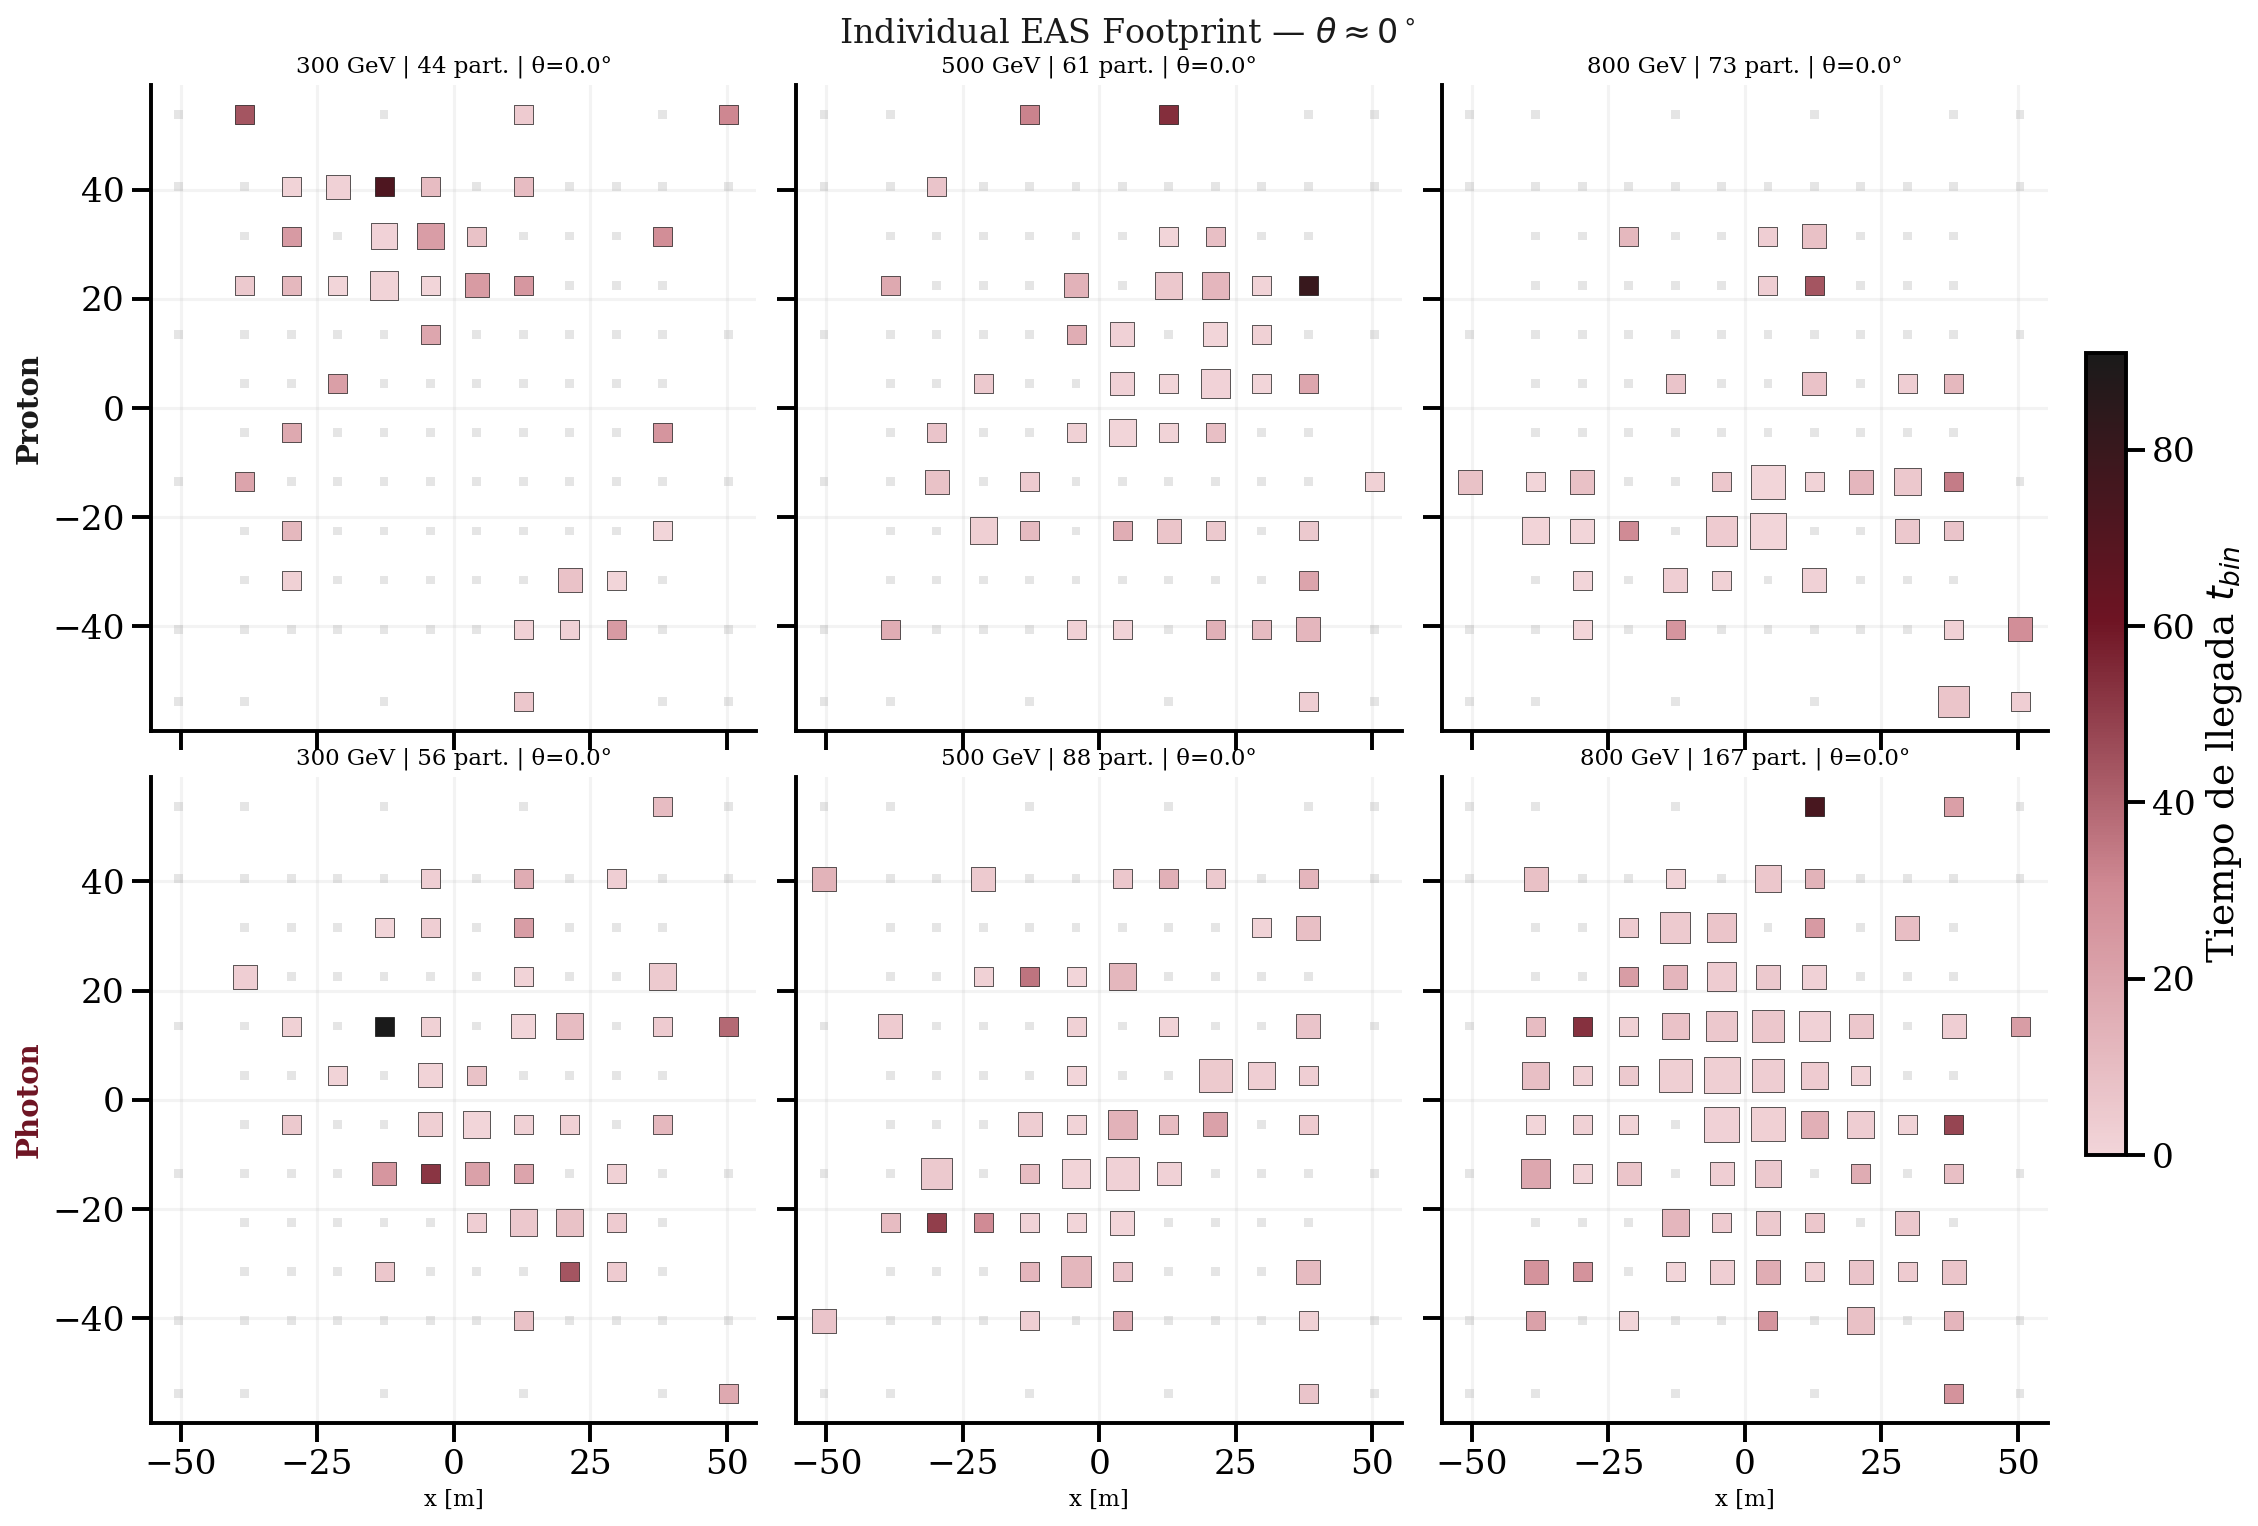
\includegraphics[width=1\linewidth]{figures/eas_individual_events.png}
    \caption[Representative individual EAS footprints by particle type and energy.]{Representative individual EAS footprints at $\theta \approx 0\degree$, for proton-induced (top row) and gamma-induced (bottom row) showers at 300, 500, and 800 GeV primary energy. Each event is selected as the one closest to the median total particle count for its group. Color encodes the arrival time $t_\mathrm{bin}$ of particles at each detector; marker size is proportional to particle count. Individual events exhibit significant stochastic fluctuations in lateral spread and hit multiplicity.}
    \label{fig:individual_events}
\end{figure}

Averaging over many events per bin removes this variability and exposes the underlying morphology. Figure~\ref{fig:footprint_grid} shows the mean footprints computed over roughly 770 events per cell: gamma-induced showers concentrate the deposited energy in a compact central core, whereas proton-induced showers spread it more widely and irregularly across the array. This morphological asymmetry is the primary discriminant the classification head learns to exploit.

\begin{figure}[!ht]
    \centering
    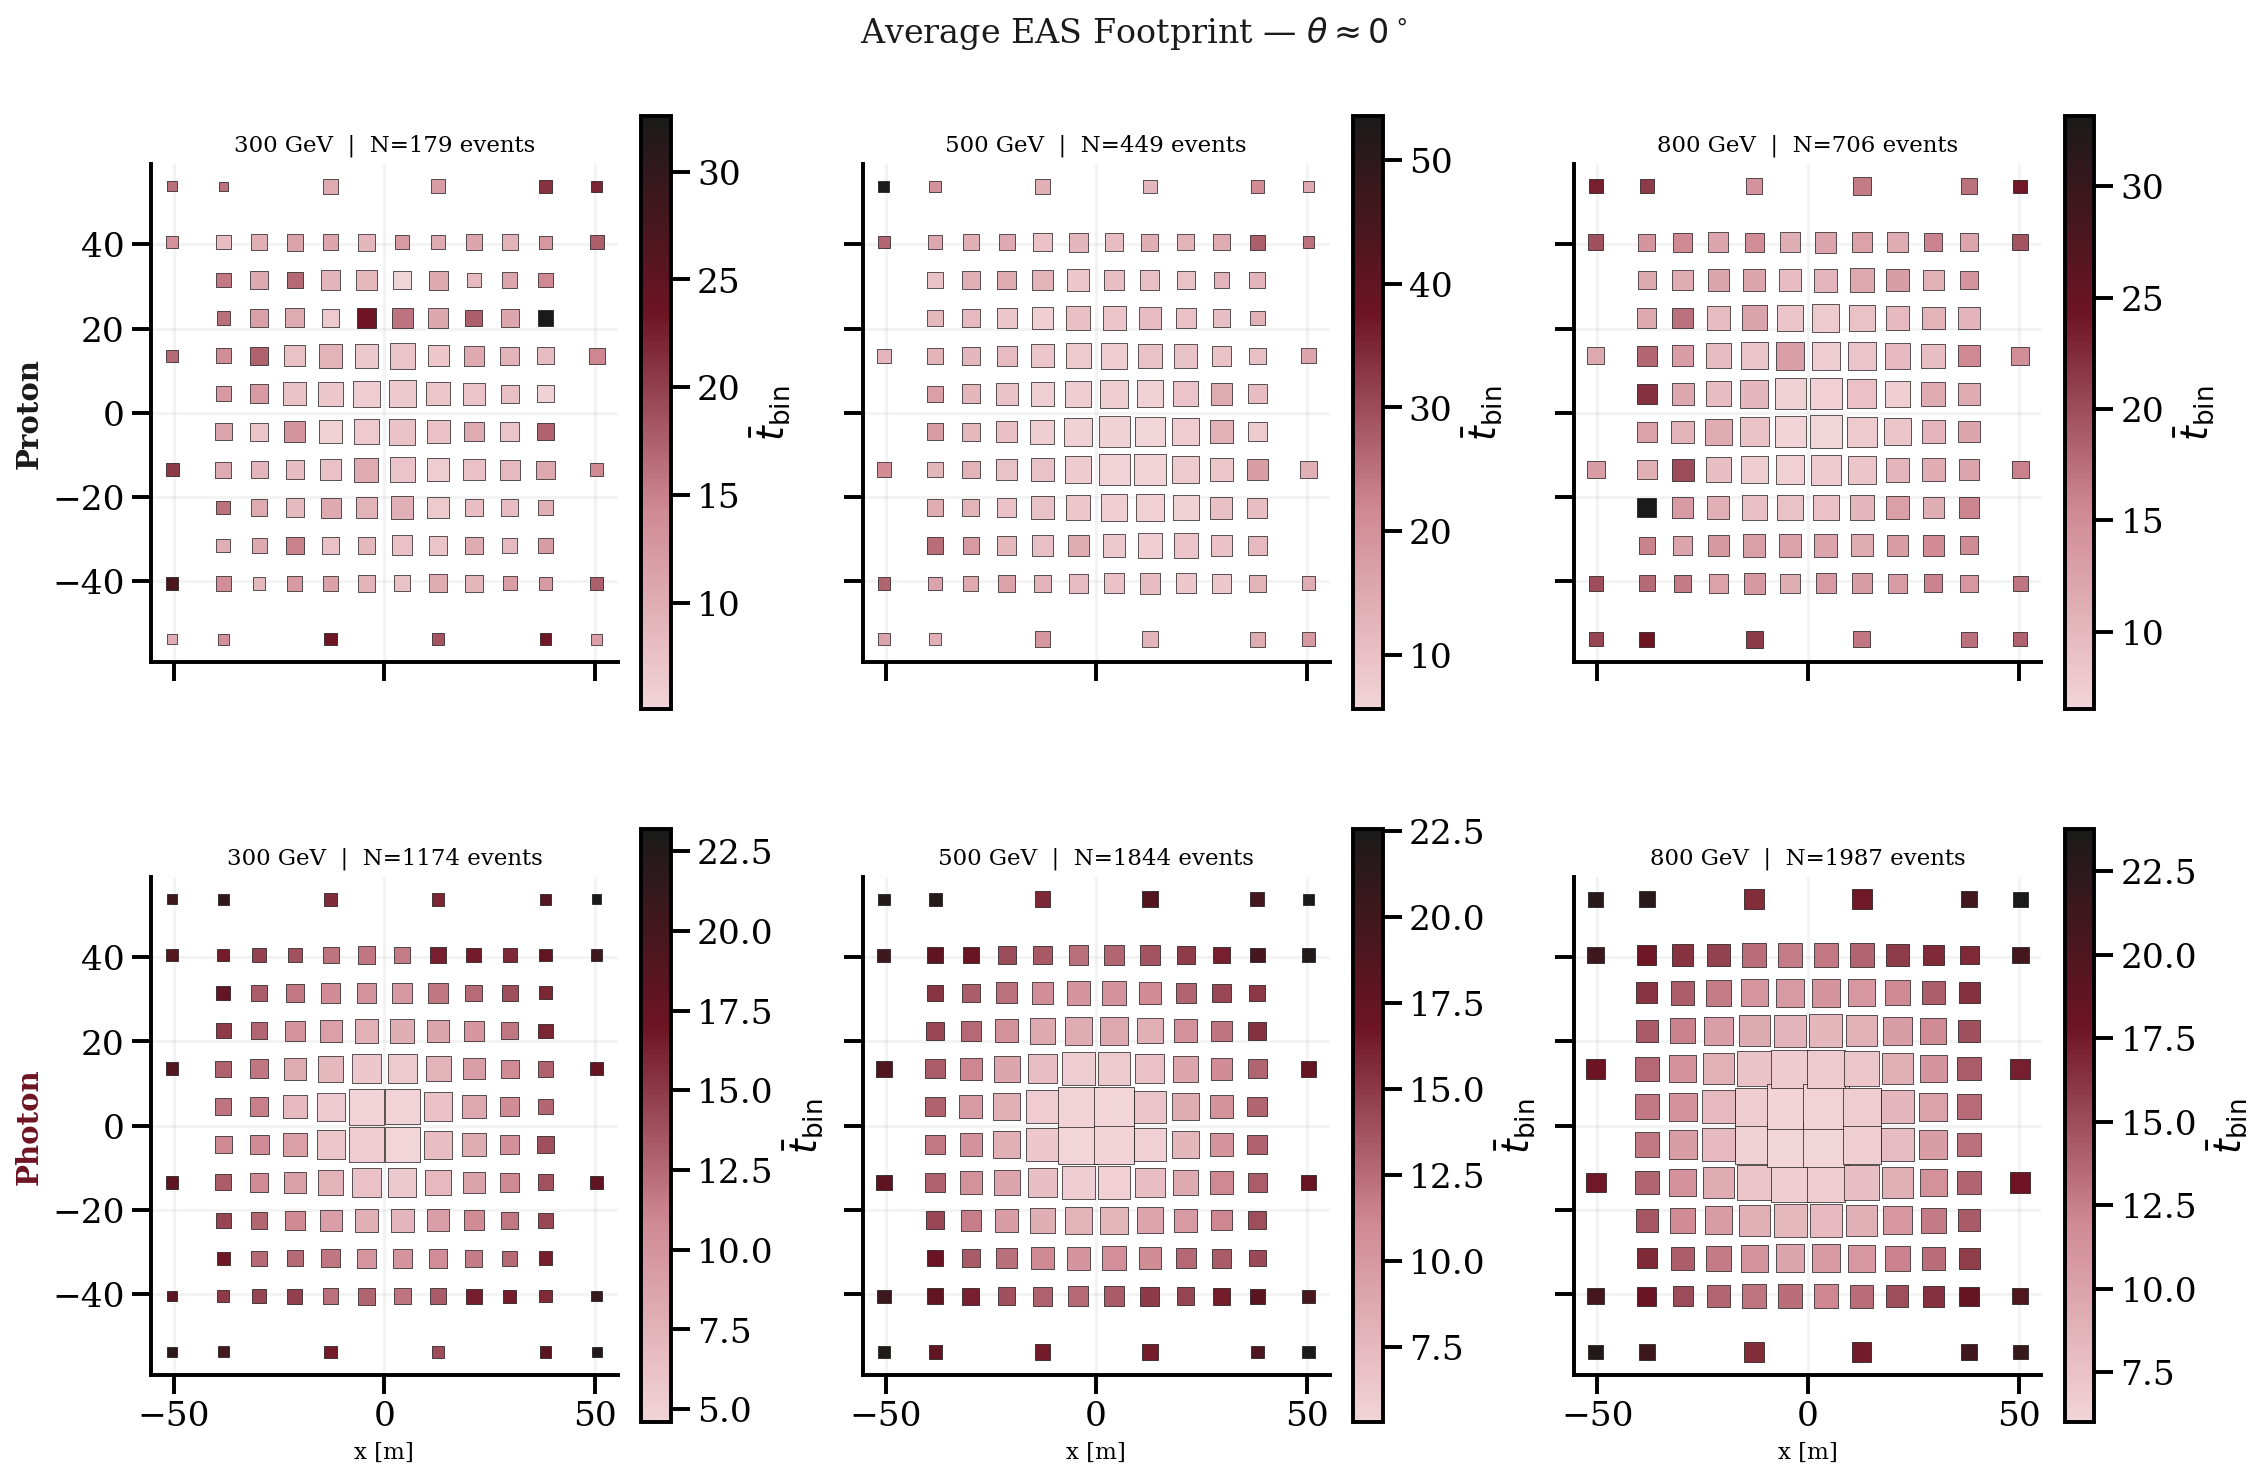
\includegraphics[width=1\linewidth]{figures/eas_footprint_grid.png}
    \caption[Average EAS footprints by particle type and energy.]{Average EAS footprints at $\theta \approx 0\degree$, computed over all events in each particle-type and energy bin (${\sim}770$ events per cell). Averaging suppresses single-event fluctuations and reveals the systematic morphological signatures of each class: gamma-induced showers produce a more compact, centrally concentrated deposit, while proton-induced showers exhibit a broader lateral spread and higher peripheral particle counts. Color encodes the mean arrival time $\bar{t}_\mathrm{bin}$; marker size is proportional to mean particle count.}
    \label{fig:footprint_grid}
\end{figure}

Both input branches are normalized before training. The sequential features are standardized channel-wise using the mean and standard deviation computed over the training set, and the global features are scaled to the unit interval using training set minimum and maximum values. Normalization statistics are computed exclusively on the training partition and applied without modification to the validation and test sets, ensuring that no information from the evaluation data influences the preprocessing.

\section{Data Stratification and Balance Strategy}

The raw simulated dataset is not uniformly distributed across the space of primary particle types, energies, and zenith angles. This imbalance arises from the interaction between the simulation configuration and the multiplicity filter: showers at large zenith angles or low energies produce fewer secondary particles at detector level on average and are therefore more frequently discarded. Left uncorrected, this imbalance would bias the shared encoder toward the conditions most heavily represented in the training data, degrading performance on underrepresented configurations and compromising the fairness of the multi-task optimization.
To address this, a stratified resampling procedure is applied before the dataset split. Let
\begin{equation}
    S = \{s_1, s_2, \ldots, s_K\}
\end{equation}
denote the set of all $K$ strata, where each stratum $s_i$ is defined by a unique combination of primary energy $E \in \{300,500,800\}$ GeV, particle type $p \in \{\text{proton}, \gamma\}$, and discretized zenith angle bin $\theta$. For each stratum $s_i$, let $n_i$ denote its event count after multiplicity filtering. The target population size is defined as
\begin{equation}
    n_\text{target} = \text{median}(\{n_1, n_2, \ldots, n_K\})
\end{equation}
which evaluates to $n_\text{target} = 593$ for this dataset. The median is preferred over the mean as a balancing objective because it is insensitive to outliers and extreme population disparities: under the median criterion, half of the strata are downsampled and half are upsampled, without being influenced by extremely large or small strata. The resampling procedure operates independently on each stratum:
\begin{equation}
n_i^{\text{balanced}} = \begin{cases}
\text{undersample}(s_i, n_{\text{target}}) & \text{if } n_i > n_{\text{target}} \\
\text{oversample}(s_i, n_{\text{target}}) & \text{if } n_i < n_{\text{target}} \\
n_i & \text{if } n_i = n_{\text{target}}
\end{cases}
\end{equation}

where undersampling randomly selects $n_{\text{target}}$ events from the $n_i$ available events without replacement, effectively removing $n_i - n_{\text{target}}$ events. Oversampling duplicates events with replacement until the stratum size reaches $n_{\text{target}}$, introducing $n_{\text{target}} - n_i$ duplicate samples. This ensures that after resampling, all strata satisfy $n_i^{\text{balanced}} = n_{\text{target}}$.

The resulting balanced dataset contains approximately 74,700 events in total. These are split into training, validation, and test partitions in a ratio of approximately 70:15:15, yielding roughly 52,300 training events, 11,200 validation events, and 11,200 test events. The split is performed after stratified resampling and maintains the balanced distribution across all three partitions. No event appears in more than one partition, and the test set is held out entirely until final evaluation. Figure~\ref{fig:data_balancing} illustrates the original event distributions per energy and the resampling target, and Table~\ref{tab:dataset_balancing} summarizes the dataset composition before and after balancing.
\begin{table}[ht!]
\centering
\caption[Dataset composition before and after balancing.]{Dataset composition before and after balancing. $\gamma$: \# gamma events, \textbf{p}: $\#$ proton events.}
\label{tab:dataset_balancing}
\begin{tabular}{cccc}
\toprule
\textbf{E (GeV)} & \textbf{$\gamma$} & \textbf{p} & \textbf{Total} \\
\midrule
\multicolumn{4}{c}{\textit{Original}} \\
300  & 14474 & 1958 & \textbf{16432} \\
500  & 27611 & 5306 & \textbf{32917} \\
800 & 36143 & 11496 & \textbf{47639} \\
\midrule
\multicolumn{4}{c}{\textit{Balanced}} \\
300  & 12453 & 12453 & \textbf{24906} \\
500  & 12453 & 12453 & \textbf{24906} \\
800  & 12453 & 12453 & \textbf{24906} \\
\bottomrule
\end{tabular}
\end{table}

Figure~\ref{fig:data_balancing} illustrates the effect of the resampling strategy across the three marginal distributions. After balancing, the label distribution is equalised between proton and gamma classes, the zenith angle distribution becomes uniform across the full $0\degree$--$40\degree$ range, and the energy distribution is balanced across the three primary energy levels. The resulting dataset satisfies $n_i^{\text{balanced}} = n_{\text{target}}$ for all $i \in \{1, \ldots, K\}$, ensuring equitable representation across all physics configurations.

\begin{figure*}[ht!]
    \centering
    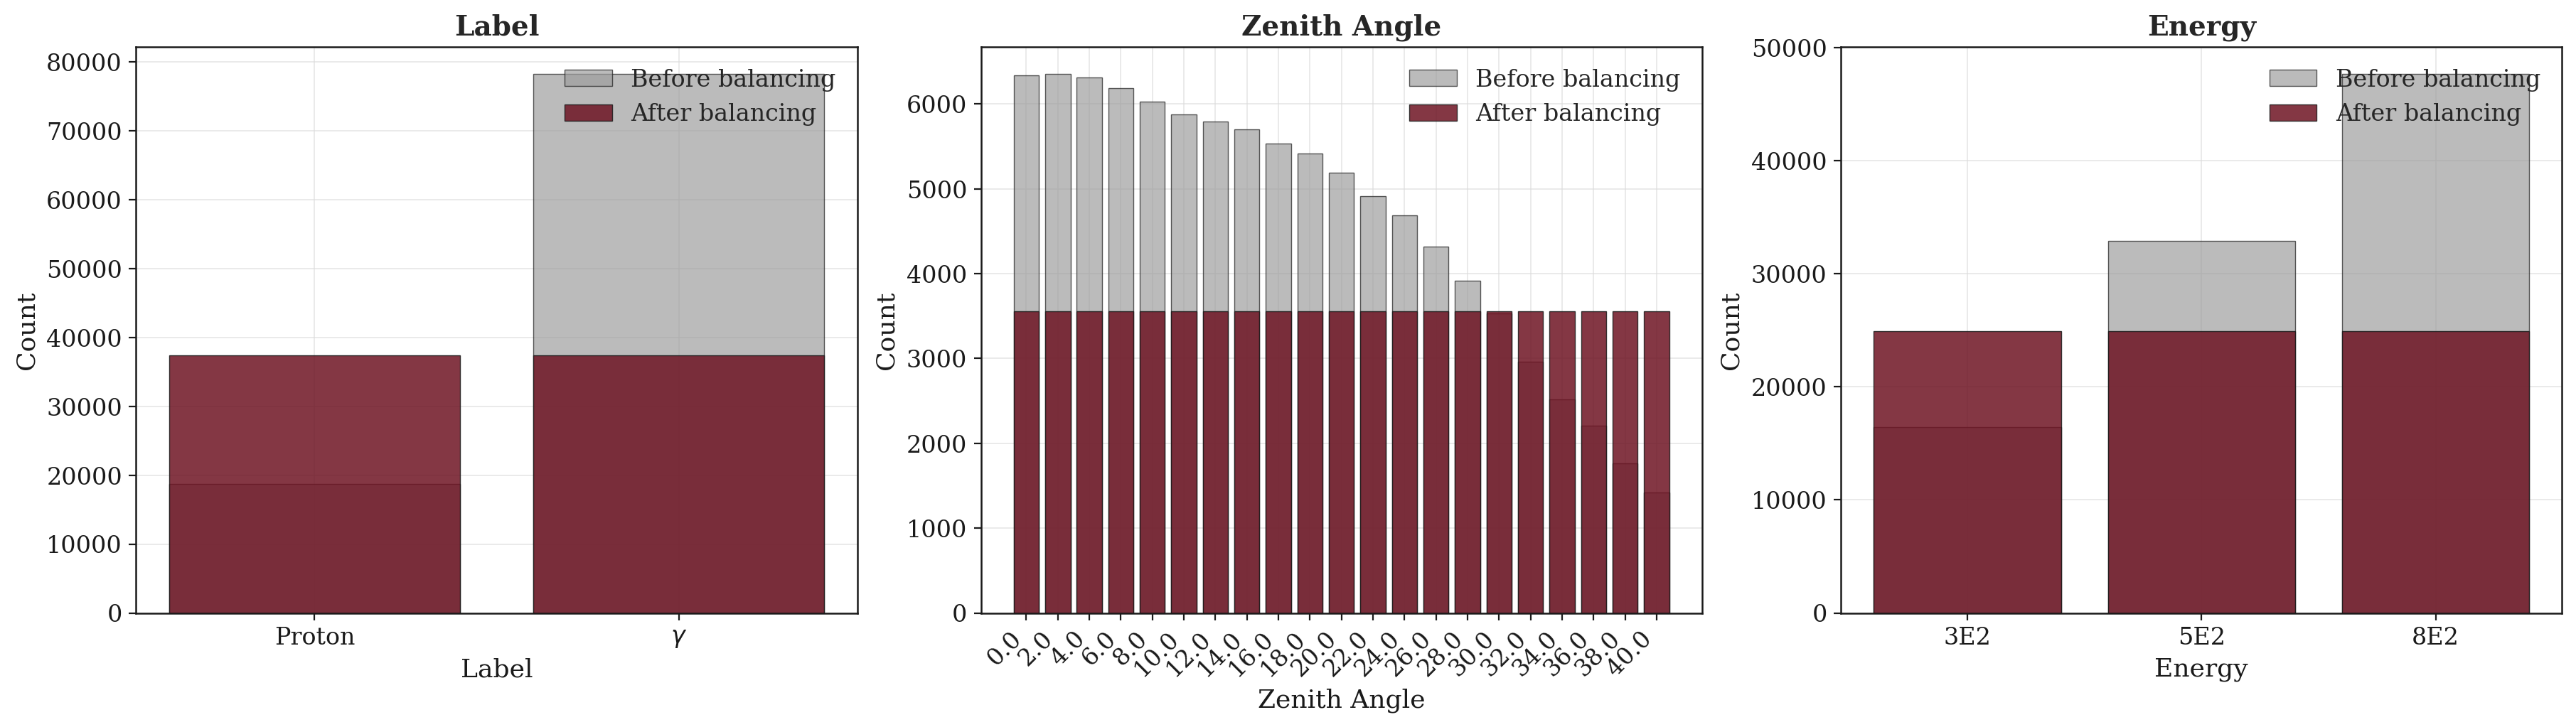
\includegraphics[width=1\linewidth]{figures/data_balancing.png}
    \caption[Event distributions before and after stratified balancing.]{Distribution of events by label, zenith angle, and primary energy before (grey) and after (dark red) stratified balancing. Grey bars extending above the dark red bars indicate categories that were undersampled to reach the median target of 593 events per stratum; categories where both bars align were already close to the target or were oversampled.}
    \label{fig:data_balancing}
\end{figure*}

This combined over- and undersampling approach ensures that each physics configuration is represented equitably during training. The final balanced dataset, whose composition by energy and particle type is summarized in Table~\ref{tab:dataset_split}, helps the model to develop unbiased decision boundaries across the entire parameter space.

\begin{table}[ht!]
\centering
\caption[Dataset composition after stratified balancing.]{Dataset composition after stratified balancing, showing the number of events by primary energy, particle type, and split. Energy labels: 3E2 = 300 GeV, 5E2 = 500 GeV, 8E2 = 800 GeV.}
\label{tab:dataset_split}
\begin{tabular}{lrrrrrrc}
\toprule
\textbf{Split} & \textbf{3E2-$\gamma$} & \textbf{3E2-p} & \textbf{5E2-$\gamma$} & \textbf{5E2-p} & \textbf{8E2-$\gamma$} & \textbf{8E2-p} & \textbf{Total} \\
\midrule
\textbf{Train}      & 8678 & 8684 & 8728 & 8718 & 8745 & 8749 & \textbf{52302} \\
\textbf{Val} & 1892 & 1894 & 1838 & 1875 & 1872 & 1836 & \textbf{11207} \\
\textbf{Test}       & 1883 & 1875 & 1887 & 1860 & 1836 & 1868 & \textbf{11209} \\
\bottomrule
\end{tabular}
\end{table}

A methodological note on the interaction between oversampling and the data split is warranted. Because the resampling procedure is applied before the split into training, validation, and test partitions, oversampled strata contain duplicated events. The splitting procedure assigns each event instance to exactly one partition, but for strata where $n_i < n_\text{target}$, different copies of the same physical event may appear in different partitions, creating a potential information leak between training and test data.

The magnitude of this effect is not negligible and is strongly class-dependent. As shown in Table~\ref{tab:dataset_balancing}, the gamma class is abundant at all three energies (78,228 events before balancing) and is therefore downsampled in every stratum, so all gamma events in the balanced dataset are unique. The proton class, by contrast, is scarce (18,760 events before balancing) and falls below the median target in every stratum, so all proton strata are oversampled. Consequently the balanced dataset contains $37{,}359 - 18{,}760 = 18{,}599$ duplicated proton instances, which amounts to roughly 25\% of the total dataset and approximately half of the proton class. Duplicate copies of a given proton event are distributed across the partitions, so a proton event in the test set frequently has an identical copy in the training set.

This asymmetry has a concrete implication for interpretation: it can selectively inflate the apparent performance on proton events. In particular, the markedly better energy resolution obtained for protons (16--18\%) compared to gammas (28--41\%, Section~\ref{subsec:energy}) is attributed below to shower physics, but a fraction of the gap could also reflect partial memorization of duplicated proton events. The gamma-class metrics are not subject to this effect, since gamma events are never duplicated. This caveat should be kept in mind when reading the per-class results. Alternative strategies that avoid the leak entirely --- performing the split before resampling, undersampling instead of oversampling, or replacing duplication with class-weighted losses or post-split augmentation --- would remove this ambiguity and represent a natural direction for future refinement.

\section{Model Architecture}

The reconstruction model is a hybrid CNN-Transformer architecture designed for multi-task learning over dual-input shower data. Its design reflects three requirements: the ability to extract local temporal features from the sequential input, the ability to model global dependencies across the full hit sequence, and the flexibility to specialize independently for each of the three reconstruction tasks without forcing a single shared representation to serve all objectives equally. A schematic diagram of the full architecture is shown in Figure~\ref{fig:flowchart}.

\textbf{CNN backbone.} The sequential input is first processed by a convolutional backbone consisting of three successive Conv1D layers, each with 128 filters, kernel size 7, same-padding, and ELU activation. Batch normalization is applied after each convolutional layer. After the third convolutional layer, a single max-pooling operation with stride 2 halves the temporal resolution before the representation is passed to the projection layers. The three-layer structure progressively expands the effective receptive field: the first layer captures local patterns within a handful of consecutive hits, while the third integrates information over a wider temporal window. The max-pooled output is then projected through three fully connected layers of dimensions 128, 256, and 128 with ELU activations, and dropout of rate 0.4 is applied after the 256-dimensional layer.

\textbf{Task-specific Transformer streams.} The architecture employs six independent Transformer streams, two per reconstruction task. For each task, one stream operates on the 128-dimensional CNN output sequence (the \textit{CNN stream}), and a second stream operates directly on the raw masked six-dimensional hit sequence (the \textit{RAW stream}). Each stream applies a single pre-norm Transformer encoder block with one attention head and key dimension $d_k = 32$, as described in Section~\ref{sec:transformer}. The CNN streams capture high-level temporal patterns abstracted by the convolutional backbone. The RAW streams attend directly to individual detector hits, enabling attention maps that can be interpreted in terms of specific physical observables, such as which detectors and time bins the model prioritizes for each task, without the indirection introduced by convolutional transformations. Using two dedicated streams per task ensures that each reconstruction objective can develop an independent attentional strategy without competing with the others for a shared mechanism.

\textbf{Fusion and output heads.} The output of each stream is summarized by global average pooling. For each task, the pooled CNN-stream vector (128 dimensions) and the pooled RAW-stream vector (6 dimensions, matching the raw feature depth) are concatenated to form a 134-dimensional fused attention representation, which is then concatenated with the five-dimensional global feature vector to yield a 139-dimensional fused representation. This representation is passed through a task-specific dense layer of 128 units with ELU activation and then mapped to the final prediction: a sigmoid-activated scalar for gamma-hadron classification and a linear-activated scalar for each regression task. Task-specific dropout is applied before the dense head, with rates of 0.35 for classification, no dropout for zenith angle regression, and 0.5 for energy estimation. The total model contains 531,375 parameters, of which 530,607 are trainable and 768 are non-trainable batch normalization statistics.

\clearpage
\begin{landscape}
    \centering
    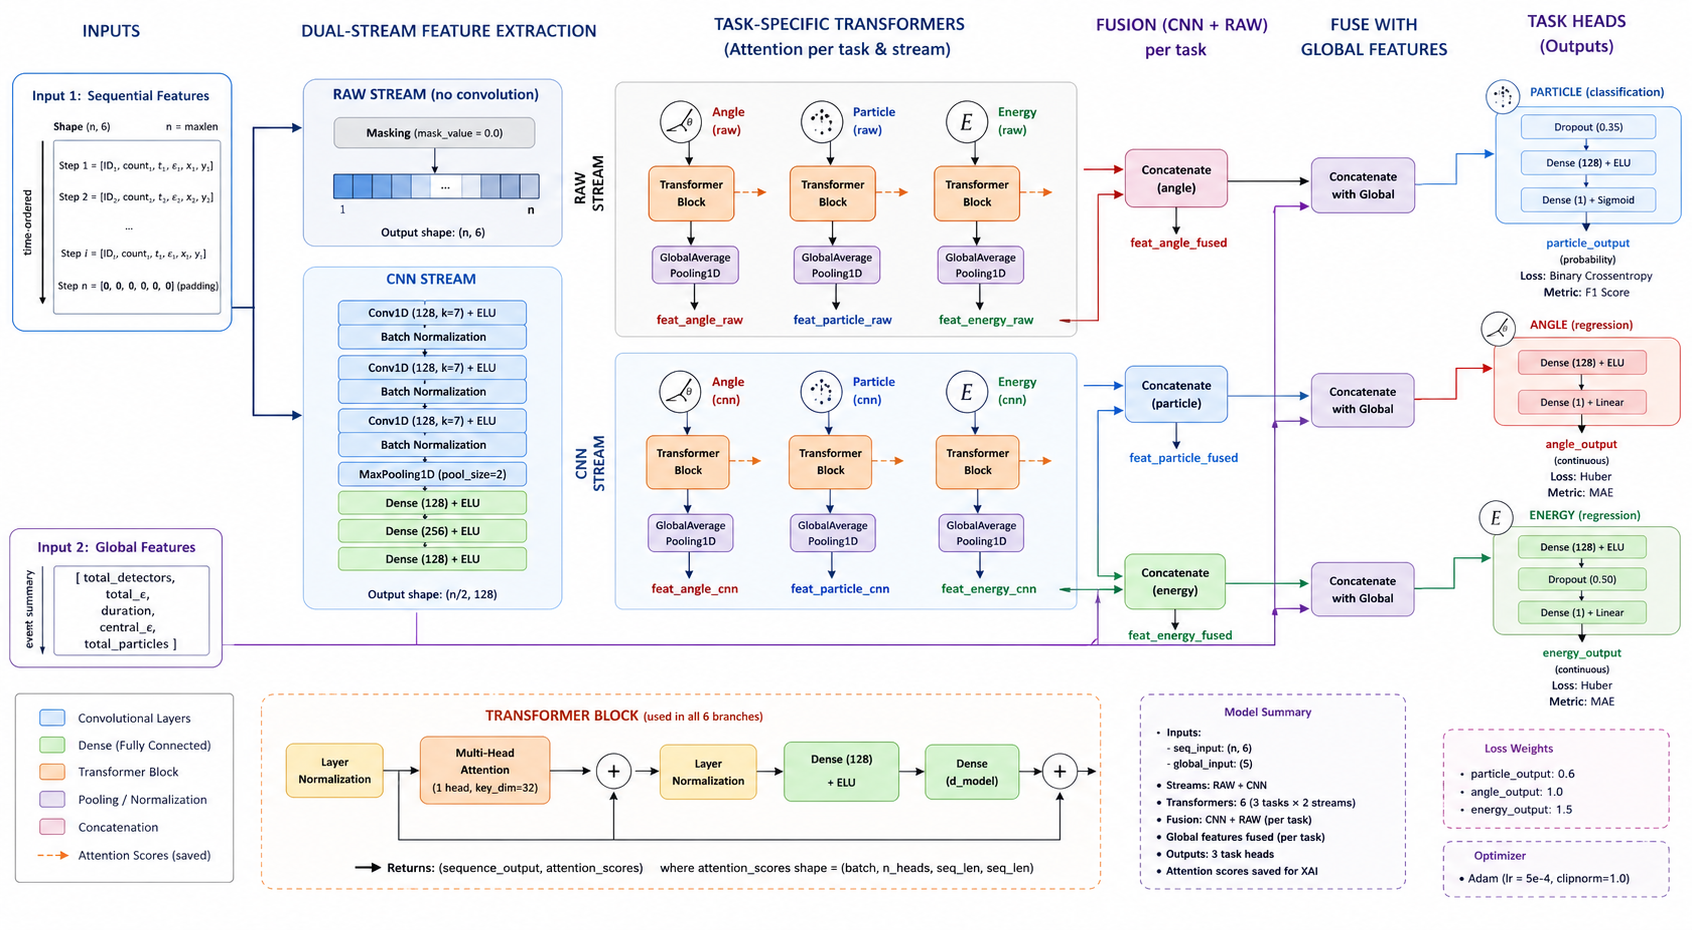
\includegraphics[width=\linewidth]{figures/flowchart_architecture.png}
    \captionof{figure}{Flow diagram of the CNN-Transformer multi-task model.}
    \label{fig:flowchart}
\end{landscape}
\clearpage

\section{Hyperparameter Optimization}
\label{sec:hyperparameter}

The model contains a number of hyperparameters that influence training dynamics and final performance, including the learning rate, task loss weights, and the dropout rates for the classification and energy heads. An initial search was conducted using Optuna~\shortcite{akiba2019optuna}, a framework for automated hyperparameter optimization based on Bayesian search with tree-structured Parzen estimators (TPE)~\shortcite{bergstra2011algorithms}. TPE models the distributions of hyperparameter configurations that lead to good and poor outcomes separately, and uses the ratio of these distributions to propose new trials that are more likely to improve the objective. This approach is substantially more sample-efficient than grid or random search, particularly when the hyperparameter space is high-dimensional.

The search space covered the learning rate over the range $[10^{-4}, 10^{-2}]$ on a logarithmic scale, the task loss weights $\lambda_\text{cls}$, $\lambda_\theta$, and $\lambda_E$ each over $[0.1, 2.0]$, and the dropout rates for the classification and energy heads independently over $[0.1, 0.6]$. Each trial trained the model for a fixed number of epochs and evaluated the combined validation loss as the optimization objective; divergent trials were pruned early using Optuna's built-in median pruner. The Optuna search provided initial estimates for the hyperparameter ranges, which were then refined through targeted manual tuning of the loss weights and dropout rates. The final configuration, reported in Table~\ref{tab:hyperparameters}, was selected based on validation performance across all three tasks simultaneously.

\begin{table}[htbp]
\centering
\caption[Consolidated hyperparameter configuration.]{Consolidated hyperparameter configuration for the final model.}
\label{tab:hyperparameters}
\footnotesize
\setlength{\tabcolsep}{7pt}
\renewcommand{\arraystretch}{1.1}
\begin{tabular}{llc}
\toprule
\textbf{Category} & \textbf{Parameter} & \textbf{Value} \\
\midrule
\multirow{3}{*}{CNN backbone}
  & Conv1D filters & 128 \\
  & Kernel size & 7 \\
  & CNN dropout & 0.4 \\
\midrule
\multirow{2}{*}{Transformer}
  & Attention heads & 1 \\
  & Key dimension $d_k$ & 32 \\
\midrule
\multirow{3}{*}{Task weights}
  & $\lambda_\text{cls}$ & 0.6 \\
  & $\lambda_\theta$ & 1.0 \\
  & $\lambda_E$ & 1.5 \\
\midrule
\multirow{3}{*}{Task dropout}
  & Classification & 0.35 \\
  & Angle & 0.0 \\
  & Energy & 0.5 \\
\midrule
\multirow{5}{*}{Training}
  & Optimizer & Adam \\
  & Learning rate & $5 \times 10^{-4}$ \\
  & Gradient clip norm & 1.0 \\
  & LR reduction patience & 7 epochs \\
  & Early stopping patience & 15 epochs \\
\midrule
\multirow{2}{*}{Data}
  & Batch size & 64 \\
  & Max sequence length & 472 \\
\bottomrule
\end{tabular}
\end{table}

The final task weights are
\begin{align*}
    \lambda_\text{cls} &= 0.6 \\
    \lambda_\theta &= 1.0 \\
    \lambda_E &= 1.5 ,
\end{align*}
reflecting the relative difficulty of each task and the need to prevent the binary classification objective from dominating the regression signals early in training.

\section{Training Configuration}

The model is trained by minimizing the weighted multi-task loss:
\begin{equation}
    \mathcal{L}_\text{total} = \lambda_\text{cls} \mathcal{L}_\text{cls} + \lambda_\theta \mathcal{L}_\theta + \lambda_E \mathcal{L}_E
\end{equation}
where $\mathcal{L}_\text{cls}$ is the binary cross-entropy loss for gamma-hadron classification and $\mathcal{L}_\theta$, $\mathcal{L}_E$ are Huber losses for zenith angle and energy regression respectively, as defined in Section~\ref{sec:multitask}. Optimization is performed using the Adam optimizer~\shortcite{kingma2015adam} with learning rate $5 \times 10^{-4}$ and gradient norm clipping at 1.0. The learning rate is reduced by a factor of 0.5 whenever the combined validation loss fails to improve for seven consecutive epochs, with a minimum learning rate floor of $10^{-6}$. This plateau reduction schedule allows the optimizer to take larger steps during the initial training phases and shift to finer adjustments as the model approaches convergence, which proved effective for balancing the three task objectives simultaneously.

Training is stopped early when the combined validation loss fails to improve for 15 consecutive epochs, and the model checkpoint achieving the lowest validation loss is restored for final evaluation. No information from the test set is used at any point during training or hyperparameter search. Table~\ref{tab:hyperparameters} consolidates all hyperparameters of the final configuration.

All experiments were conducted on a single NVIDIA GeForce RTX 3050 Ti Laptop GPU (4 GB VRAM) using TensorFlow 2.10 with CUDA 11.2. A full training run to convergence (61 epochs, with the best checkpoint at epoch 46) required approximately 45 minutes. The total model contains 531,375 parameters, of which 530,607 are trainable and 768 are non-trainable batch normalization statistics.